\subsection{Weigths}

Um die Bewegung des Gittergraphen �ber den Skelett genau zu kontrollieren k�nnen wir jeden Punkt isoliert betrachten. F�r jeden einzelnen Punkt k�nnen wir festlegen, wie er auf Bewegungen des Skeletts reagieren soll. So k�nnen wir zum Beispiel bestimmen, dass ein Punkt auf dem Ellenbogen eines Menschen sich bewegen soll, wenn Oberarm oder Unterarm sich bewegen, oder dass er sich zwar bewegen soll, aber anders als andere Punkte. So k�nnte man zum Beispiel definieren, dass Punkte sich immer weniger bewegen sollen, je n�her sie einem anderen Knochen kommen. Diese Kontrolle �ber die Bewegung eines Punktes nennt sich Gewichte.


\begin{figure}[t]
		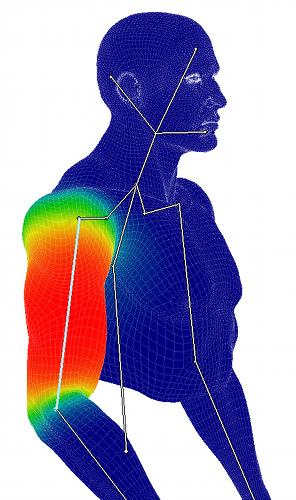
\includegraphics[width=7cm]{01_Skinning/pics/weight.png}
		\caption[Fl�chige Gewichtsverteilung]{ Modelldarstellung der fl�chigen Gewichtsverteilung auf einem Mesh. Die Farben beschreiben die Verteilung der Gewichte auf einer Skala von Blau=0, damit unabh�ngig, zu Rot=1, damit komplett abh�ngig. Entnommen von \cite{weights}}
		\label{weights_fig1}
\end{figure}

Gewichte bezeichnen, wie abh�ngig ein Punkt auf dem Gittergraphen bei einer Transformation von einem Knochen ist. Sie sind die L�sung, um bei verformbarem Material abzusch�tzen, inwiefern sich jeder Punkt auf der Haut beeinflussen l�sst. Dieses Gewicht $wi$ in Relation zu Knochen $i$, ist $0<=wi<=1$. Wobei 0 komplett unabh�ngig von dem Knochen und 1 komplett von dem Knochen abh�ngig ist. So w�re zum Beispiel ein Punkt auf dem Oberarm des Knochen diesem komplett mit einer 1 zugeh�rig, ein Punkt an der H�fte h�tte ein Gewicht von 0 am Oberarm und w�re damit komplett unabh�ngig von diesem. Gewichte von Punkten am Ellbogengelenk h�tten variierende Werte zwischen 0 und 1. 

Nun k�nnten wir f�r jeden Vertex eine Liste  mit allen seinen Gewichten in Bezug auf jeden Knochen erstellen, um zusammengefasst darzustellen, wie ein Punkt sich durch das Skelett bewegen l�sst. In der Summe entsprechen alle seine Gewichte immer 1, ergo $\sum_{i=1}^{N}wi=1$. Dies ist darin begr�ndet, dass das Material der Haut im Normalfall eine konstante Beweglichkeit aufweist. H�tte ein Punkt eine h�here Summe an Gewichten als ein anderer, w�rde dies darauf hindeuten, das er sich leichter und von mehr Knochen bewegen lie�e. Nat�rlich wird nicht jeder Punkt eines Modells in der Animation gleich verformt, dies ist dann aber darauf zur�ckzuf�hren, dass Knochen des zu Grunde liegenden Skelettes weniger bewegt werden, woraufhin die Knochen, die in Verbindung mit ihnen gebracht werden, proportional zu ihrem Gewicht weniger Bewegung erfahren. Zum Beispiel ein Punkt am Bauch wird wesentlich weniger bewegt werden als Punkte an den Extremit�ten. 

Um Gewichte zuzuordnen k�nnen verschiedene Verfahren angewandt werden, unter anderem Distanz-basierte Algorithmen oder durch L�sung eines "{}least squares problems"{} \cite{wang2002multi}. Oft ist es jedoch am effektivsten, wenn durch K�nstler auf Grundlage anatomischer Kenntnisse die Gittergraphen selber nach Gewichten einf�rbt werden \cite{LectureA}.

Ein recht interessanter Ansatz ist jedoch hier \cite{embedding} zu finden. Die Autoren standen vor dem selben Problem, dass Gewichte in der Regel manuell vergeben werden, wollten aber einen automatischen Ansatz verwenden. Werden die Gewichte automatisch nach N�he zu Knochen verteilt, kann dies zu Problem f�hren. So w�rden zum Beispiel Punkte auf dem Oberk�rper, an welchen ein Arm eng anliegt, hohe Gewichte auf dem Oberarmknochen erhalten, obwohl dieser Knochen sie wahrscheinlich minimal beeinflusst. Stattdessen wird in diesem Paper Gewicht wie Hitze behandelt, welche sich gleichm��ig �ber die Oberfl�che verteilt, wie auf Abbildung 10 zu sehen.

\begin{figure}[t]
	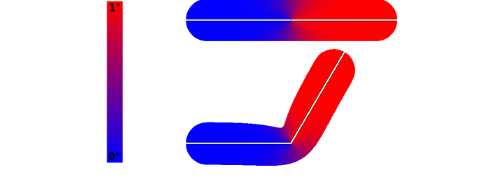
\includegraphics[width=7cm]{01_Skinning/pics/heat.png}
	\caption[Hitze Equilibrium zur Gewichtsverteilung]{ Hitze Gleichgewicht an zwei Knochen. Entnommen von \cite{embedding}}
	\label{heat_fig1}
\end{figure}

Es wird angenommen, dass bei Knochen $i$ die Hitze 1 ist, bei allen anderen Knochen 0. Dann bestimmen wir das Gewicht jedes Punktes zu Knochen $i$ als seine Hitze. Dieses Vorgehen basiert auf Basis eines Hitzegleichgewichts. Der in diesem Paper entwickelte Algorithmus wird inzwischen weit verbreitet in der Industrie eingesetzt. Zum Beispiel bei der bekannten Software Blender. 



